\thispagestyle{empty}\SourceLeaf{7}
\pdfbookmark[0]{Werke. Band II}{half-title}
\begin{center}
\vspace*{1.8in}
{\Large CARL FRIEDRICH GAUSS WERKE\par}
\vspace{.5in}
{\large BAND II.\par}
\end{center}
\clearpage
\thispagestyle{empty}\SourceLeaf{9}
\pdfbookmark[0]{Zweiter Abdruck. 1876}{volume-title}
\begin{center}
{\Large CARL FRIEDRICH GAUSS\par}
\vspace{.35in}{\Huge WERKE\par}
\vspace{.35in}{\large ZWEITER BAND.\par}
\vspace{.2in}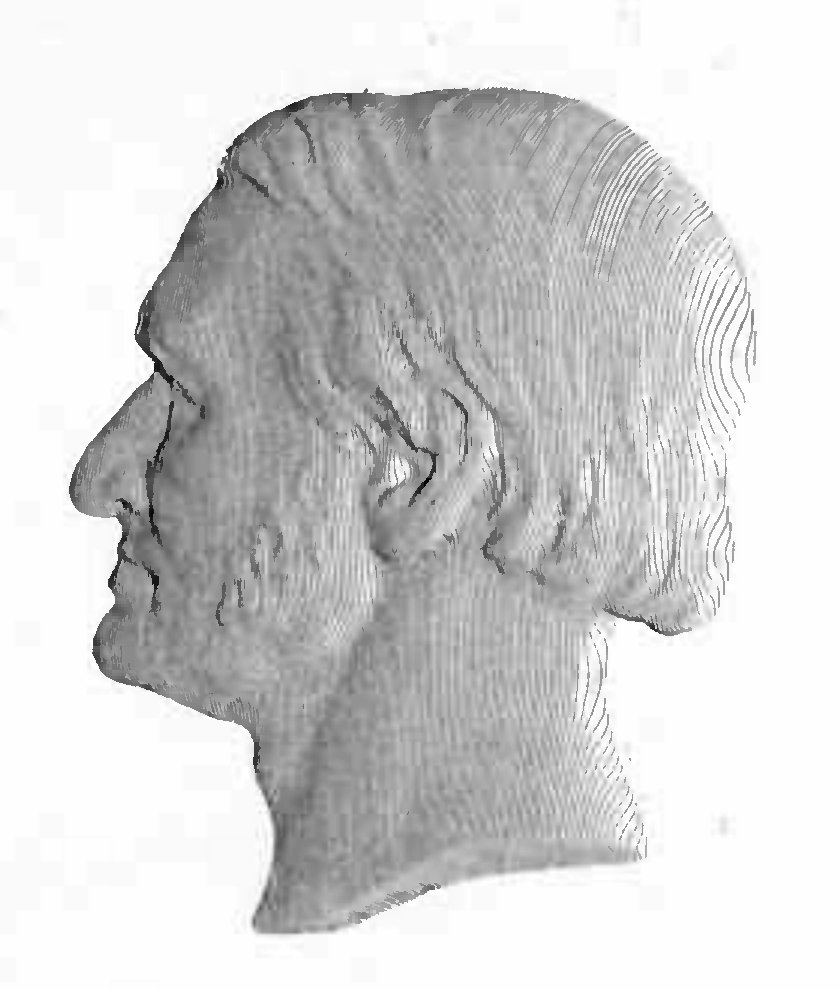
\includegraphics[width=1.6in]{assets/title_profile_contrast.png}\par
\vspace{.3in}{\large ZWEITER ABDRUCK\par}
\vspace{.2in}HERAUSGEGEBEN\par
\smallskip{\small VON DER\par}
\medskip{\small KÖNIGLICHEN GESELLSCHAFT DER WISSENSCHAFTEN\par}
\smallskip{\small ZU\par}
\medskip{\large GÖTTINGEN\par}
\smallskip1876.
\end{center}
\clearpage
\thispagestyle{empty}\SourceLeaf{11}
\pdfbookmark[0]{Ein neuer Beweis eines arithmetischen Satzes}{paper-one-title}
\begin{center}
\vspace*{.8in}
{\Large EIN NEUER BEWEIS\par}
\bigskip{\large EINES ARITHMETISCHEN SATZES\par}
\vspace{.6in}VON\par
\bigskip{\large CARL FRIEDRICH GAUSS\par}
\vspace{.3in}{\small DER KÖNIGLICHEN GESELLSCHAFT DER WISSENSCHAFTEN VORGELEGT AM 15. JANUAR 1808.\par}
\vspace{.65in}\rule{.85\linewidth}{.3pt}\par
\smallskip{\small Commentationes societatis regiae scientiarum Gottingensis. Vol. \textsc{xvi}.\par}
{\small Gottingae \textsc{mdcccviii}.\par}
\smallskip\rule{.85\linewidth}{.3pt}
\end{center}
\clearpage
